\section{Data Exploration}

\subsection{Importing the FakeNewsCorpus dataset.}
The first challenge was simply downloading and unpacking the files on our Linux systems. We ended up concatenating the
files into a temporary zip file using \texttt{cat} and then unzipping the file using \texttt{unzip}. \\

Trying to read the data in python proved to be a challenging task, as the .csv file seemed to be corrupted or malformed with rows containing different amounts of columns. Some article content included \texttt{\textbackslash r}, which was interpreted as "newline", and thus, a new row in the middle of arbitrary news content. A single command '\texttt{sed 's/\textbackslash r/ /g' in.csv > out.csv}' replacing the carriage returns with spaces (to preserve word boundaries) turned out to solve this issue.\\
% \todo{Perhaps missing a section on summary statistics?}

\subsection{Larger than memory datasets}
Due to the size of our dataset, we had to use different methods for handling our data. Throughout this report we used 3 different methods: SQL Databases, chunk-wise operations and brute force (acces
to a large enough server). After getting the data into a readable CSV file in the previous step, we decided to load it
into an SQL database for easier handling and exploration. In later sections we will use the other two methods as they
are more appropriate for specific machine learning tasks.


\subsubsection{Summary of the dataset}
In this section we'll present some summary statistics. The dataset contains $ 8.528.956 $ articles. The articles are
sorted into the following categories: [bias, clickbait, conspiracy, fake, hate, junksci (junk science), political,
reliable, rumor, satire, unknown, unreliable]. The number of articles in each category is distributed as seen in figure
\ref{fig:combdist}. The dataset contains many articles from just a few publishers, as can be seen in figure \ref{fig:combdist}.

\begin{figure}[htpb]
  \centering
  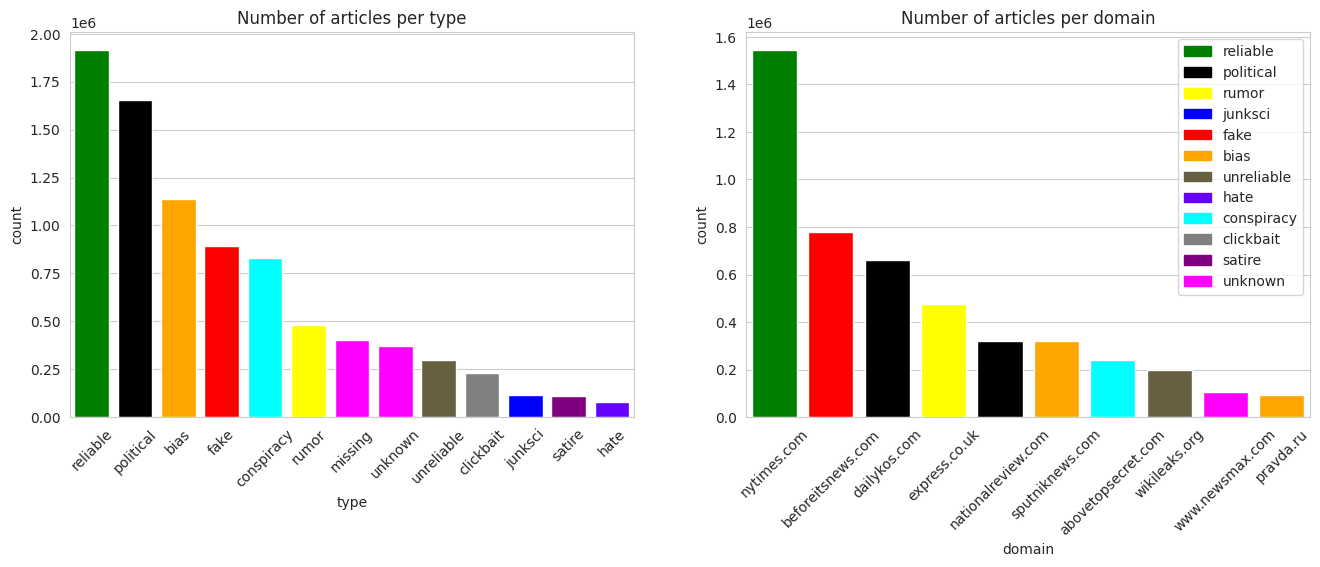
\includegraphics[width=1\textwidth]{combdist}
  \caption{Article type and domain distribution}
  \label{fig:combdist}
\end{figure}
\subsubsection{Vocabulary sizes}
After getting the data into a managable format, we were then able to start properly TK THIS SENTENCE IS WEIRD exploring it. We started by
calculating the vocabulary size of the dataset. We did this by first tokenising the data, and then counting the
unique tokens. We then repeated this process after removing stopwords, and finally after stemming the tokens. The
results are shown in table \ref{tab:vocab_sizes}. As we can see the vocabulary decreases slightly after removing
stopwords, and significantly after stemming. As we see, removing a list of common words doesn't reduce the vocabulary
much, but reducing words to their root does.

\begin{table}[h]
    \centering
    \begin{tabular}{r| c | c | c| c}
      Data& vocabulary size & vocabulary size (lowered) & \% decrease & \% decrease (lowered)\\
        \hline
      Sample data& 21016 & 18011 & 0\% & 0\% \\
    \hline
      Removed stopwords & 20674 & 17865 & 1.63\% & 0.81\% \\
    \hline
      Stemmed & 12654 & 12703 & 39.8\% & 29.5\%
    \end{tabular}
    \caption{Vocabulary sizes}
    \label{tab:vocab_sizes}
\end{table}

% TODO ADD THESE NUMBERS TO TABLE


\subsubsection{Classifiyng truth per. domain}\label{sec:truth_pr_domain}
A central aspect of the dataset, is the way it classifies news articles in terms of reliability. The creators of the
dataset has chosen to classify the articles per domain, meaning that all the articles from any given domain will be
given the same level of credibility.

\subsubsection{Duplicated articles}\label{sec:dup_articles}
Another things we realised quite quickly, is that the dataset contains a significant amount of duplicated articles as
seen in table \ref{tab:dupart}.

\begin{table}[htpb]
  \centering
  \caption{Duplicated articles and their domain}
  \label{tab:dupart}
  \begin{tabular}{r | c | c| c| c}
      domain & type & content & count&\% of corpus \\ \hline
      nationalreview.com & political & Plus one article on Google Plus (Thanks to al... & 273388 & 3.2\%\\ \hline
      wikileaks.org & unreliable & Tor Tor is an encrypted anonymising network t... & 169259 & 2.0\% \\ \hline
      sputniknews.com & bias & Dear readers, we are excited to announce that ... & 102671 & 1.2\%\\
    \multicolumn{5}{c}{$\vdots$}
  \end{tabular}
\end{table}
As we can see, this is due to different popups that the webscraper has encountered as it
was trying to scrape the dataset. These duplicated articles were simply removed before we trained our model.

\subsubsection{Lower dimensionality exploration WIP}
We have made a 2D UMAP representation of the dataset, which is a form of non-linear dimensionality reduction. We've
trained the model unsupervised to get the inherent distribution of the data without any labelling bias.
\begin{figure}[htpb]
  \centering
  \includegraphics[width=0.8\textwidth]{figures/umapFakeNewsClasses}
  \caption{UMAP representation}
  \label{fig:umap_explore}
\end{figure}

The plot, figure \ref{fig:umap_explore} contains a large cluster which contains a rough mix of everything which UMAP
couldn't separate as well as some more concentrated cluster of junk science and conspiracy articles. On the boundaries
of this cluster, we have some more concentrated clusters that the model was able to separete, this includes reliable,
fake. Away from the main cluster, we have a large cluster of almost entirely reliable content the model was easily able
to separate from everything else, other clusters far apart include unreliable and rumors. This serves as our justication for our binary grouping of the dataset since realiable articles are clearly delineated from the rest of the dataset. 



